% !TEX root=./report.tex

\subsection{Static calibration}
In the following we evaluate the implemented static calibration algorithm and assess the algorithmic and systematic errors.

\subsubsection{Systematic Error}

\begin{figure*}[t]
    \centering
    \begin{tabular}{cc}
      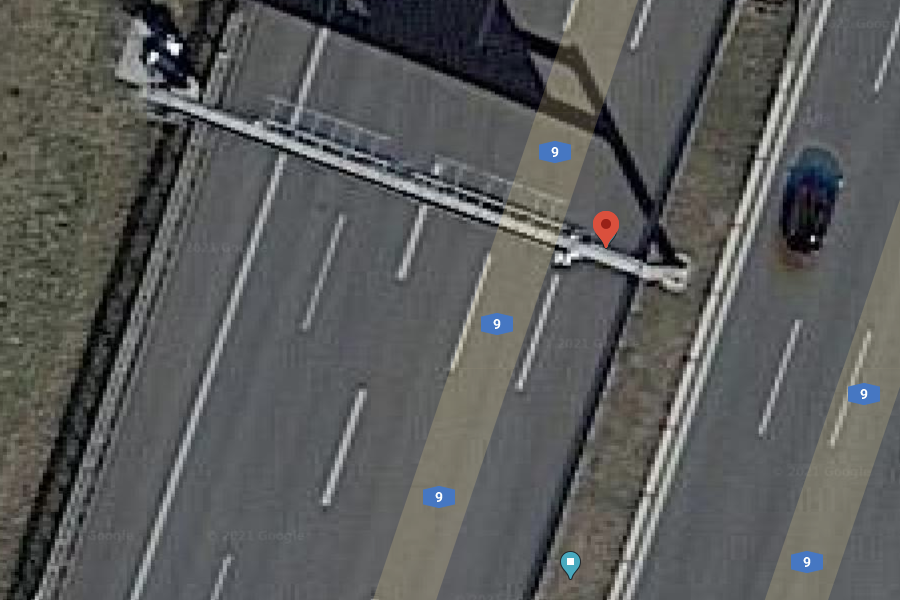
\includegraphics[width=0.45 \linewidth]{images/calibration/google_maps_s50_s.png} &
      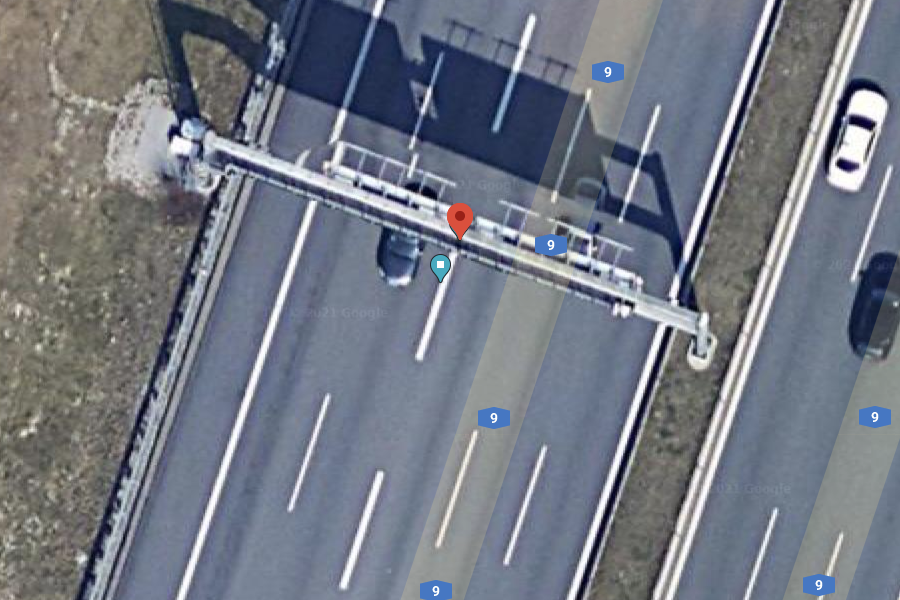
\includegraphics[width=0.45 \linewidth]{images/calibration/google_maps_s40_n.png} 
  \end{tabular}
  \caption{Left: The positions of the cameras \camsn{4} (red) and \camsf{4} (green) and their respective looking directions (yellow). 
  Right: The positions of the cameras \camsn{5} (red) and \camsf{5} (green) and their respective looking directions (yellow). 
  It displays that the rotation of the cameras is in a reasonable range so that the cameras look along the highway as expected. 
  Also the cameras are within reasonable translational bounds around their real world location as \autoref{sec:static_calibration_expectable_error} shows.
  }
  \label{fig:google_maps}
  \end{figure*}

The proposed pose estimation algorithm from \autoref{eq:static_calibration_error} converges to a pair of optimal translation $T$ and rotation $R$ values for the camera pose.
These $T, R$ values approximate the projection from the world objects to the pixels as described in \autoref{eq:static_calibration_reprojection}.

Using a maps provider we assured that the resulting values are within reasonable ranges and that there are no systematic errors in the optimization.
The results are displayed in \autoref{fig:google_maps}

\subsubsection{Expectable Error Bounds}
\label{sec:static_calibration_expectable_error}



































\subsubsection{Algorithmic Error}
The proposed pose estimation algorithm is based on the minimization of the reprojection-error \autoref{eq:static_calibration_reprojection}.
As with all optimization problems convergence is reached when the values that are optimized don't change anymore.

The optimization jointly optimizes for the 6 camera parameters, 3 for the translation, 3 for the Euler angle rotation and one $\lambda$ parameter per correspondence.
The resulting high-dimensional problem exceeds multiple minima, whereas each represents a configuration for the camera pose that well explains the dependency between pixels, world objects and the camera. 

\paragraph{Remaining Correspondences Error}
We derive a rough scale for the remaining loss over the correspondences and $\lambda$s, as only a small subset of solution are valid and represent the real camera pose.

\begin{equation}
  \label{eq:static_calibration_correspondence_error}
  \begin{split}
  E(P, S, T, R, \Lambda, W ) \simeq &
  \sum_{c \in C} 
  \left\lVert 
     p_c - \pi(T * R * s_c) 
  \right\rVert_2^2  \\
  = & 
  \sum_{c \in C} 
  \left\lVert 
     p_c - \hat{p}_c 
  \right\rVert_2^2 
  \end{split}
\end{equation}
where $p_c - \hat{p}_c$ is the remaining distance of actual pixel to the projected pixel.

The projected $\hat{p}_c$ can only be along the center line of the object due to the approximation of objects as lines.
The actual pixels $p_c$ will be evenly distributed around the center line, as we expect the objects to be roughly cylindrical (\autoref{sec:static_calibration_line_approximation}).

This implies that for a valid camera pose the remaining distance $p_c - \hat{p}_c$ can be at most half of the pixel width $w_s$ of the object (the maximal pixel distance from the center line).

It thus follows \autoref{eq:static_calibration_correspondence_error} 
\begin{equation}
  \label{eq:static_calibration_correspondence_error_scale}
  \begin{split}
  E(P, S, T, R, \Lambda, W ) \simeq  &
  \sum_{c \in C} 
  \left\lVert 
     p_c - \hat{p}_c 
  \right\rVert_2^2 \\
  = & 
  \sum_{o \in O} 
  \sum_{c_o \in C_o} 
  \left\lVert 
     p_{c_o} - \hat{p}_{c_o} 
  \right\rVert_2^2 \\
  \leq &
  \sum_{o \in O} \left\lvert C_o \right\rvert \frac{w_o}{2} 
  \end{split}
\end{equation}
where $h_o$ is the pixel height of the object.

This implies that an upper bound for the remaining error is only dependent on the number of all pixels of the objects and their respective width.
We have empirically seen that $w_0$ in our case does not exceed 10 pixels, thus the remaining error cannot exceed 
\begin{equation}
  \sum_{o \in O} \left\lvert C_o \right\rvert \frac{10}{2} = 5 * \sum_{o \in O} \left\lvert C_o \right\rvert = 5 * \left\lvert C \right\rvert 
\end{equation}
This shows that the remaining error has to be roughly in the same scale as the number of pixels over all objects. 

\paragraph{Expectable Deviations among Estimations}
As stated previously the loss landscape does exhibit a multitude of local minima, thus the optimization procedure converges to different sets of parameters. 

\begin{figure}[t]
  \centering
  \begin{tabular}{cc}
    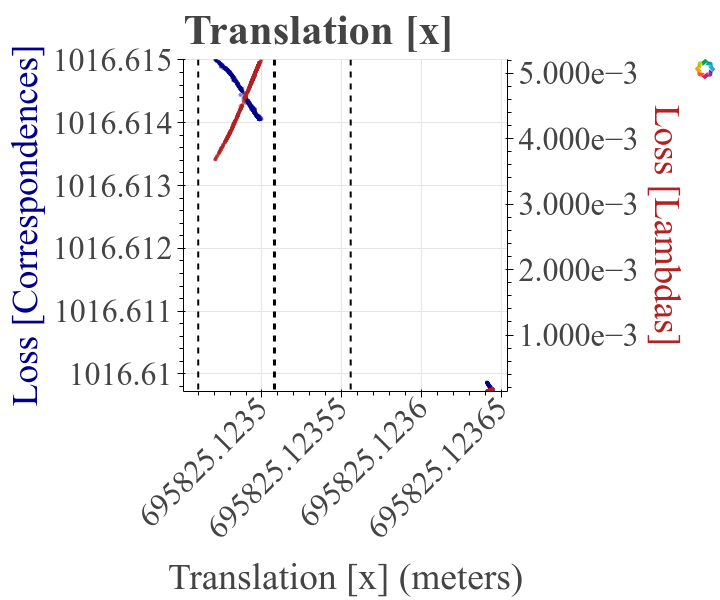
\includegraphics[width=0.45 \linewidth]{diagrams/calibration/s40_n_far_small/parameters_all.csv/Translation[x]_vs_Loss[Correspondences]_vs_Loss[Lambdas]_cluster_All.png} &
    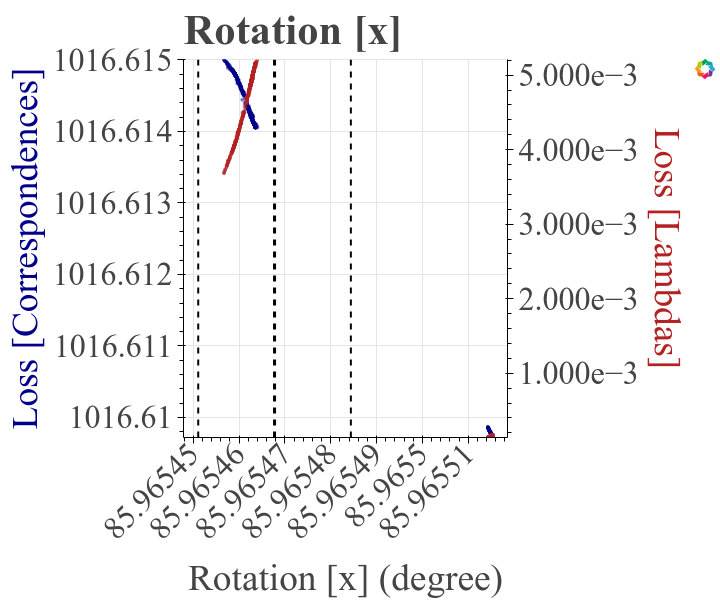
\includegraphics[width=0.45 \linewidth]{diagrams/calibration/s40_n_far_small/parameters_all.csv/Rotation[x]_vs_Loss[Correspondences]_vs_Loss[Lambdas]_cluster_All.png} \\
    
    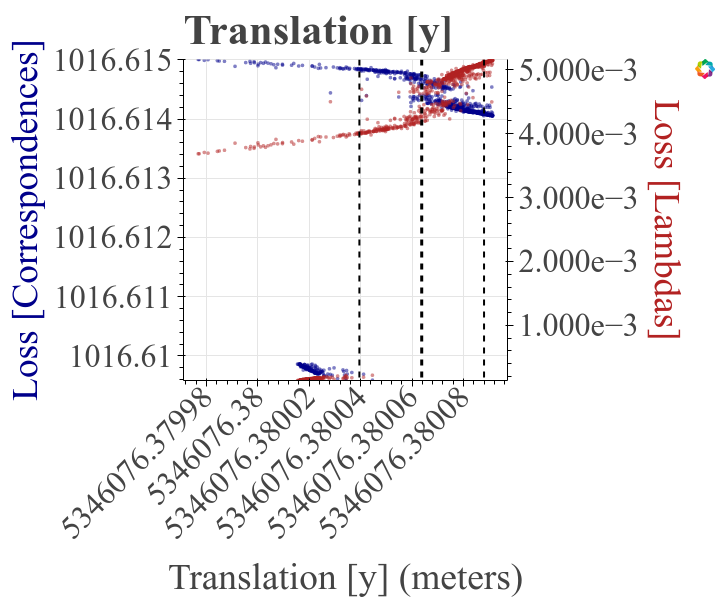
\includegraphics[width=0.45 \linewidth]{diagrams/calibration/s40_n_far_small/parameters_all.csv/Translation[y]_vs_Loss[Correspondences]_vs_Loss[Lambdas]_cluster_All.png} &
    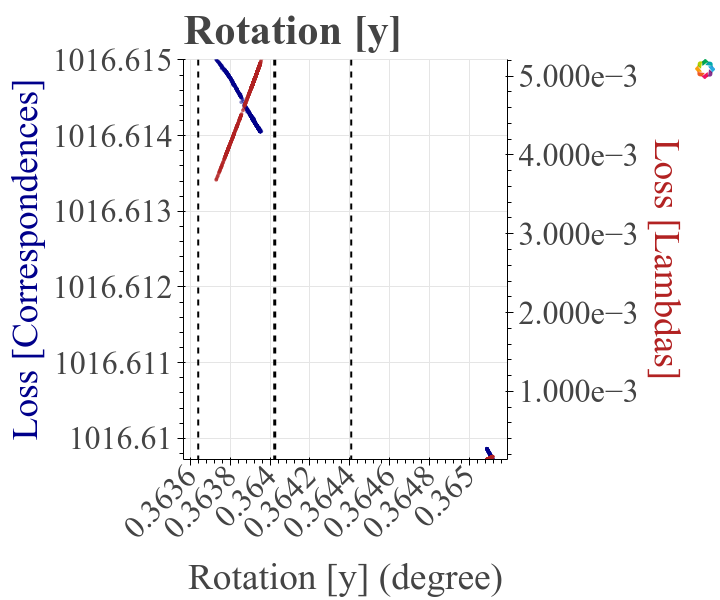
\includegraphics[width=0.45 \linewidth]{diagrams/calibration/s40_n_far_small/parameters_all.csv/Rotation[y]_vs_Loss[Correspondences]_vs_Loss[Lambdas]_cluster_All.png} \\
    
    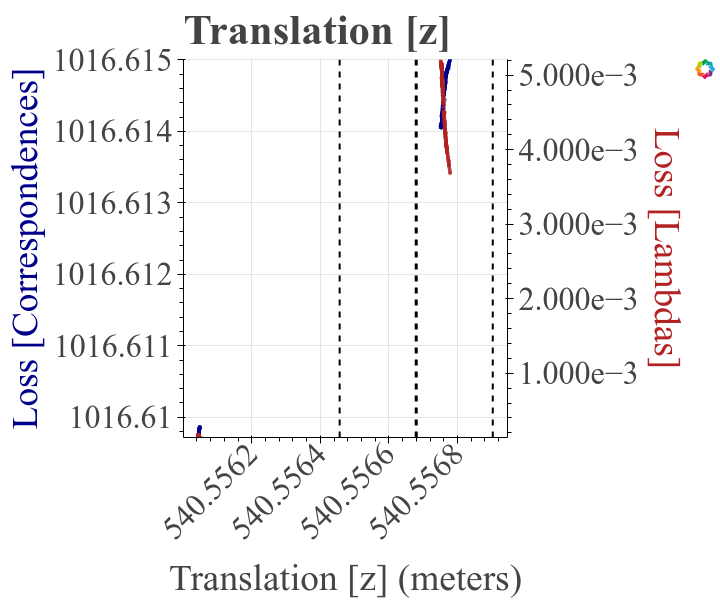
\includegraphics[width=0.45 \linewidth]{diagrams/calibration/s40_n_far_small/parameters_all.csv/Translation[z]_vs_Loss[Correspondences]_vs_Loss[Lambdas]_cluster_All.png} &
    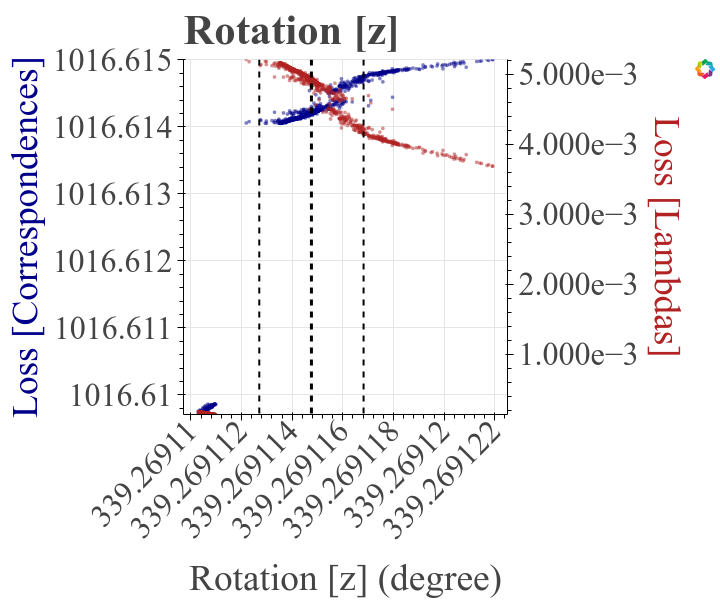
\includegraphics[width=0.45 \linewidth]{diagrams/calibration/s40_n_far_small/parameters_all.csv/Rotation[z]_vs_Loss[Correspondences]_vs_Loss[Lambdas]_cluster_All.png} \\
\end{tabular}
\caption{
  Left: The resulting translational parameters plotted against the remaining losses. 
  Right: The resulting rotational parameters plotted against the remaining losses.
  The mean of the distributions is displayed as thick dashed line. The smaller dashed lines display the standard deviation $\sigma$.
  The $\sigma$ of the translations does not exceed $2 * 10^{-4} m = 0.2 mm$.
  For the rotation $\sigma$ is at most $4 * 10^{-4} deg$.
  }
\label{fig:static_calibration_algorithmic_error}
\end{figure}

\autoref{fig:static_calibration_algorithmic_error} displays the resulting parameters for the camera \camsf{4}.
We plot the loss of the correspondence residuals and the $\lambda$ residual blocks against each of the parameters.
The translation parameters are in meters and relative to the transverse mercator projection \cite{lambert1894anmerkungen}.
The rotation parameters are in degree of Euler angles.

The plots show that the standard deviation $\sigma$ of the translations does not exceed $2 * 10^{-4} m = 0.2 mm$.
For the rotation $\sigma$ is at most $4 * 10^{-4} deg$. 

We have shown the expectable error for the parameters resulting from the sensor and map inaccuracies in \autoref{sec:static_calibration_expectable_error}. 
We conclude that in relation to these the algorithmic error can be neglected.

In the appendix \autoref{sec:appendix} we additionally evaluate the other cameras.

% \subsubsection{Minimal number of correspondences}
